\documentclass[
  letterpaper, % page size
  fontsize=10pt, % base font size
  twoside=true,
  chapterentrydots=true, % in the TOC, puts dots between name and page number
  numbers=noenddot,
  fontmethod=tex,
]{kaobook}

\usepackage[english]{babel}
\usepackage[english=british]{csquotes}

% \usepackage{kaobiblio}
% \addbibresource{handbook.bib}

\usepackage[framed=true]{kaotheorems}

\usepackage{kaorefs}

\usepackage{lib/regulation}

\graphicspath{{images/}}
%\graphicspath{{deep/path/images/}{images/}}

\makeindex[columns=3,title=Alphabetical Index,intoc]

% \makeglossaries
% \newglossaryentry{computer}{
	name=computer,
	description={is a programmable machine that receives input, stores and manipulates data, and provides output in a useful format}
}

% Glossary entries (used in text with e.g. \acrfull{fpsLabel} or \acrshort{fpsLabel})
\newacronym[longplural={Frames per Second}]{fpsLabel}{FPS}{Frame per Second}
\newacronym[longplural={Tables of Contents}]{tocLabel}{TOC}{Table of Contents}



\makenomenclature

% Reset sidenote counter at chapters
%\counterwithin*{sidenote}{chapter}

\begin{document}

% \titlehead{Displayed Top-Left on title page}
% \subject{Displayed under title}

\title[ECCC Race Handbook]{
  Collegiate Race Handbook \\
  Eastern Collegiate Cycling Conference
}
\subtitle{A comprehensive guide}

\author{Flyyn Leonard}
\date{\today}

\publishers{Northeast Collegiate Cycling Corporation}


\frontmatter

% TODO: opening page
% TODO: copyright page

\maketitle

% TODO: preface

% -------------------------------------------
% Table of Contents & Lists of Figures/Tables
% -------------------------------------------

\begingroup
\setlength{\textheight}{230\hscale} % Manually adjust height of TOC pages

% Turn on compatibility mode for etoc package
\etocstandarddisplaystyle
\etocstandardlines

\tableofcontents

\listofregulations

\listoffigures

% \listoftables

% \listoflstlistings

\endgroup

\mainmatter
\setchapterstyle{kao}

\pagelayout{wide}
\addpart{Introduction}
\pagelayout{margin}

% TODO: image is stretched, fix
\setchapterimage[7cm]{IMG_7884.jpg}
\setchapterpreamble[u]{\margintoc}
\chapter{Road Race Play-By-Play}
\labch{road-play-by-play}

This chapter will walk through the brainstorming,
planning, setup, execution, and post-event paperwork and tasks for a hypothetical collegiate road race weekend.%
\footnote{For a similar play-by-play description of a mountain race weekend,
see \nrefch{mtb-play-by-play}}

This chapter attempts to be generic, and should be applicable for both
\nrefsec{hosting:conference} and
\nrefsec{hosting:team}.
% TODO: better reference (name first)

\section{Brainstorming}

Before you can start any paperwork or other preparations,
you need to have a general idea of where you want to race.

% TODO: move to MTB play-by-play
%This is very easy for most mountain bike races -
%you must have a suitable mountain (with elevation) for downhill races,
%and Enduro and Dual Slalom races require suitable elevation and specific trails to be successful.

\subsection{Location}

The rough location of a race (at the scale of county, or rough area of a state)
is often an important decision.

Consider the following:

\begin{enumerate}
  \item Distance for collegiate students
  \item Non-collegiate race audience
  \item Local teams that could host or otherwise contribute to the race
  \item If lodging is available nearby
\end{enumerate}

\subsection{Course Design}
\index{course design}

\section{Planning and Paperwork}

After determining a general location of the race,
there are a large number of decisions to make,
services to hire,
and paperwork to complete.

\section{Course Preparation}

In the final weeks and days before the race,
some final preparations may need to be physically completed on the course.

\subsection{Notifying Residents}

\subsection{Signs}
\index{course supplies!signage}

You may need to put up No Parking signs along the course.
% TODO: legal notes

Additionally, you may consider adding local advertising signs,
directional signs to parking and the race course, and more.

\subsection{Preparing Barriers}
\index{course supplies!barriers}

\subsection{Towing}
\index{towing}

Especially for criteriums, % TODO: ref
cars on course can be extremely dangerous for participants.

Even if No-Parking signs % ref
are put up on course, local residents are still highly likely to park on course,
and towing should always be expected.

\begin{marginfigure}
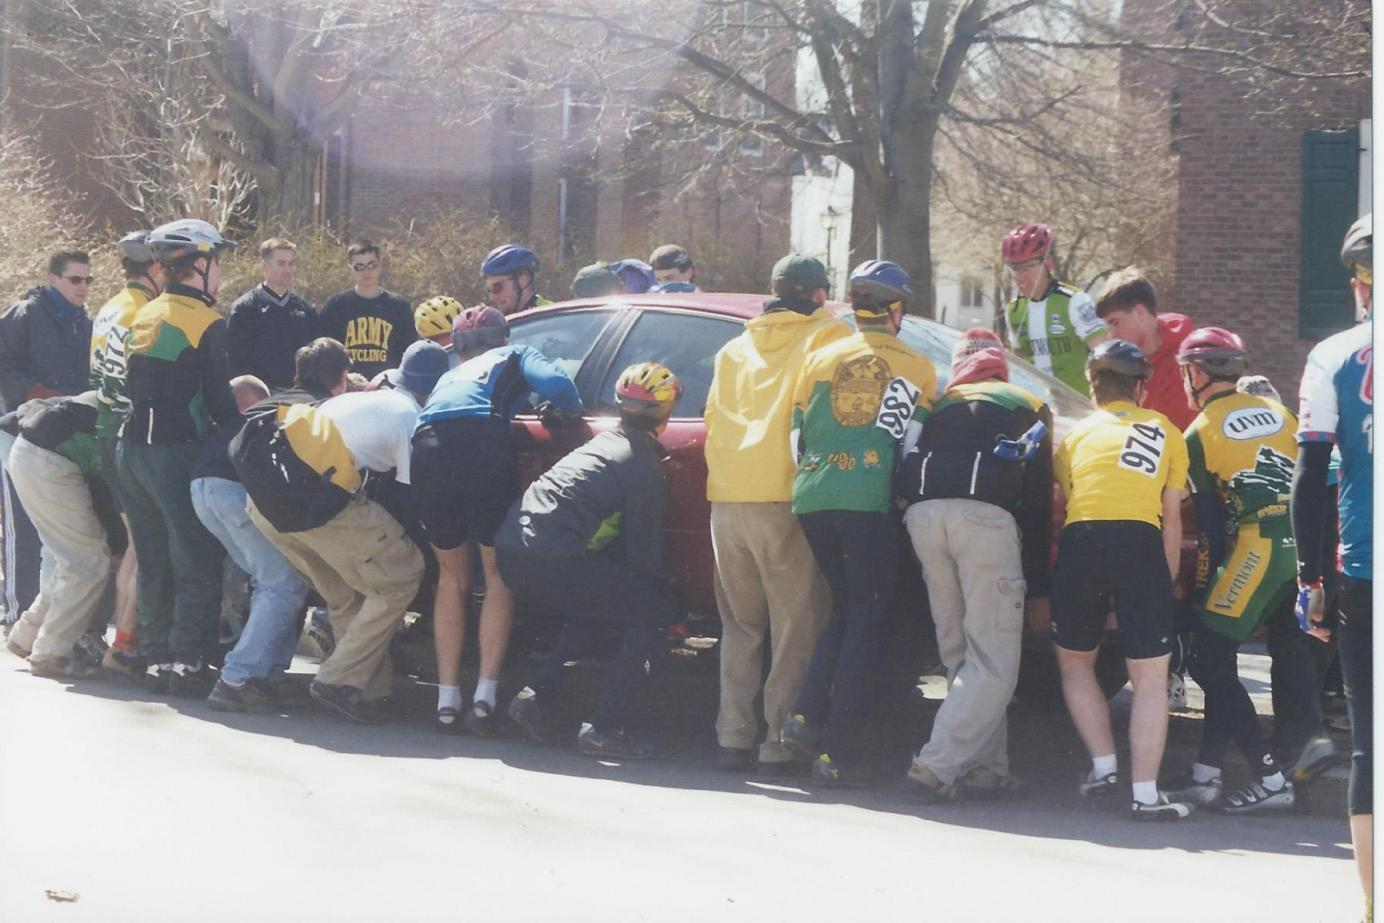
\includegraphics{dartmouth_car.jpg}
\caption[Students moving a car off a criterium course]{
          Students moving a car off of the Darmouth criterium course
          when towing services were unavailable.\\
          Credit: Alan Atwood}
\labfig{dartmouth_car}
\end{marginfigure}

% TODO: legal info?

\section{Race Weekend}

The night before the race will be upon you sooner than you expect;
hopefully all of the preparations above will have been completed!

This section will walk through all the work that needs to be done for each of the days of racing.

For this example a hypothetical schedule is described with a criterium on Saturday and both a time-trial and road race scheduled for Sunday.
Weekends may look different from this example.

Additionally, a few example medical emergencies are described
(based on actual emergencies that have happened during ECCC events).

Keep in mind that emergencies may happen at any point in time -
a rider pre-riding before a race may crash and tie up all medical services before an event even has started!

% TODO: document getting hotels for race staff

\subsection{Saturday Morning Setup}

In the very early morning (\reffig{early_am_setup})
the final setup will begin.

\begin{marginfigure}[-10pt]
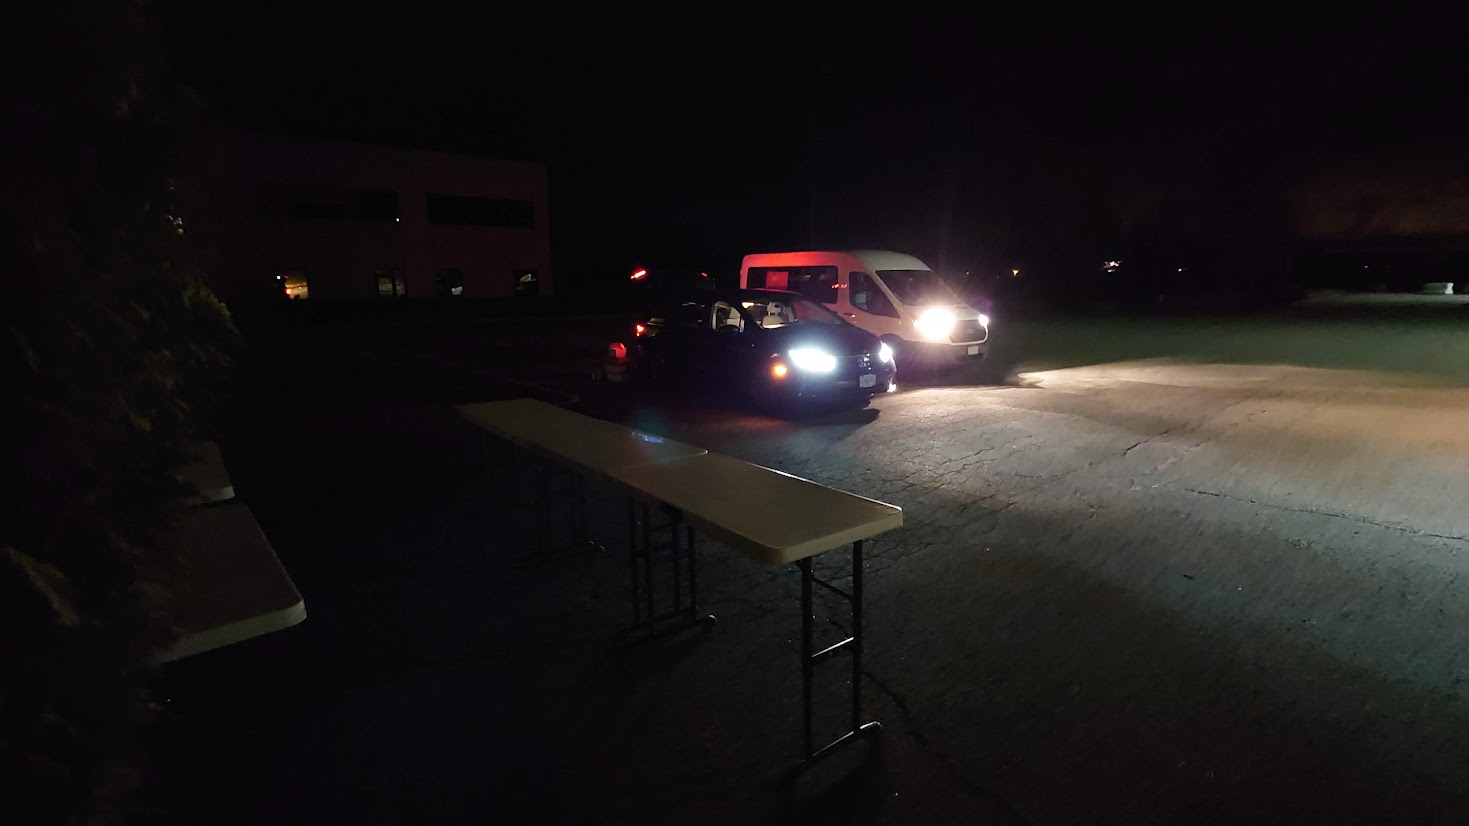
\includegraphics{2022_umass_early_am.jpg}
\caption[Early morning race setup]{Expect to be setting up well before sunrise.\\
          Credit: Flyyn Leonard}
\labfig{early_am_setup}
\end{marginfigure}

\index{registration table}
Place tables and chairs for registration,
% TODO: a better description of ideal registration location should be written elsewhere, and referenced
ideally under an ECCC branded tent (shown in \reffig{eccc_tent}). % TODO: replace with an image of a registration setup
Depending on the setup, you may also need power,
computers, boxes for paperwork, blank forms, a printer, and more.

\begin{marginfigure}[60pt]
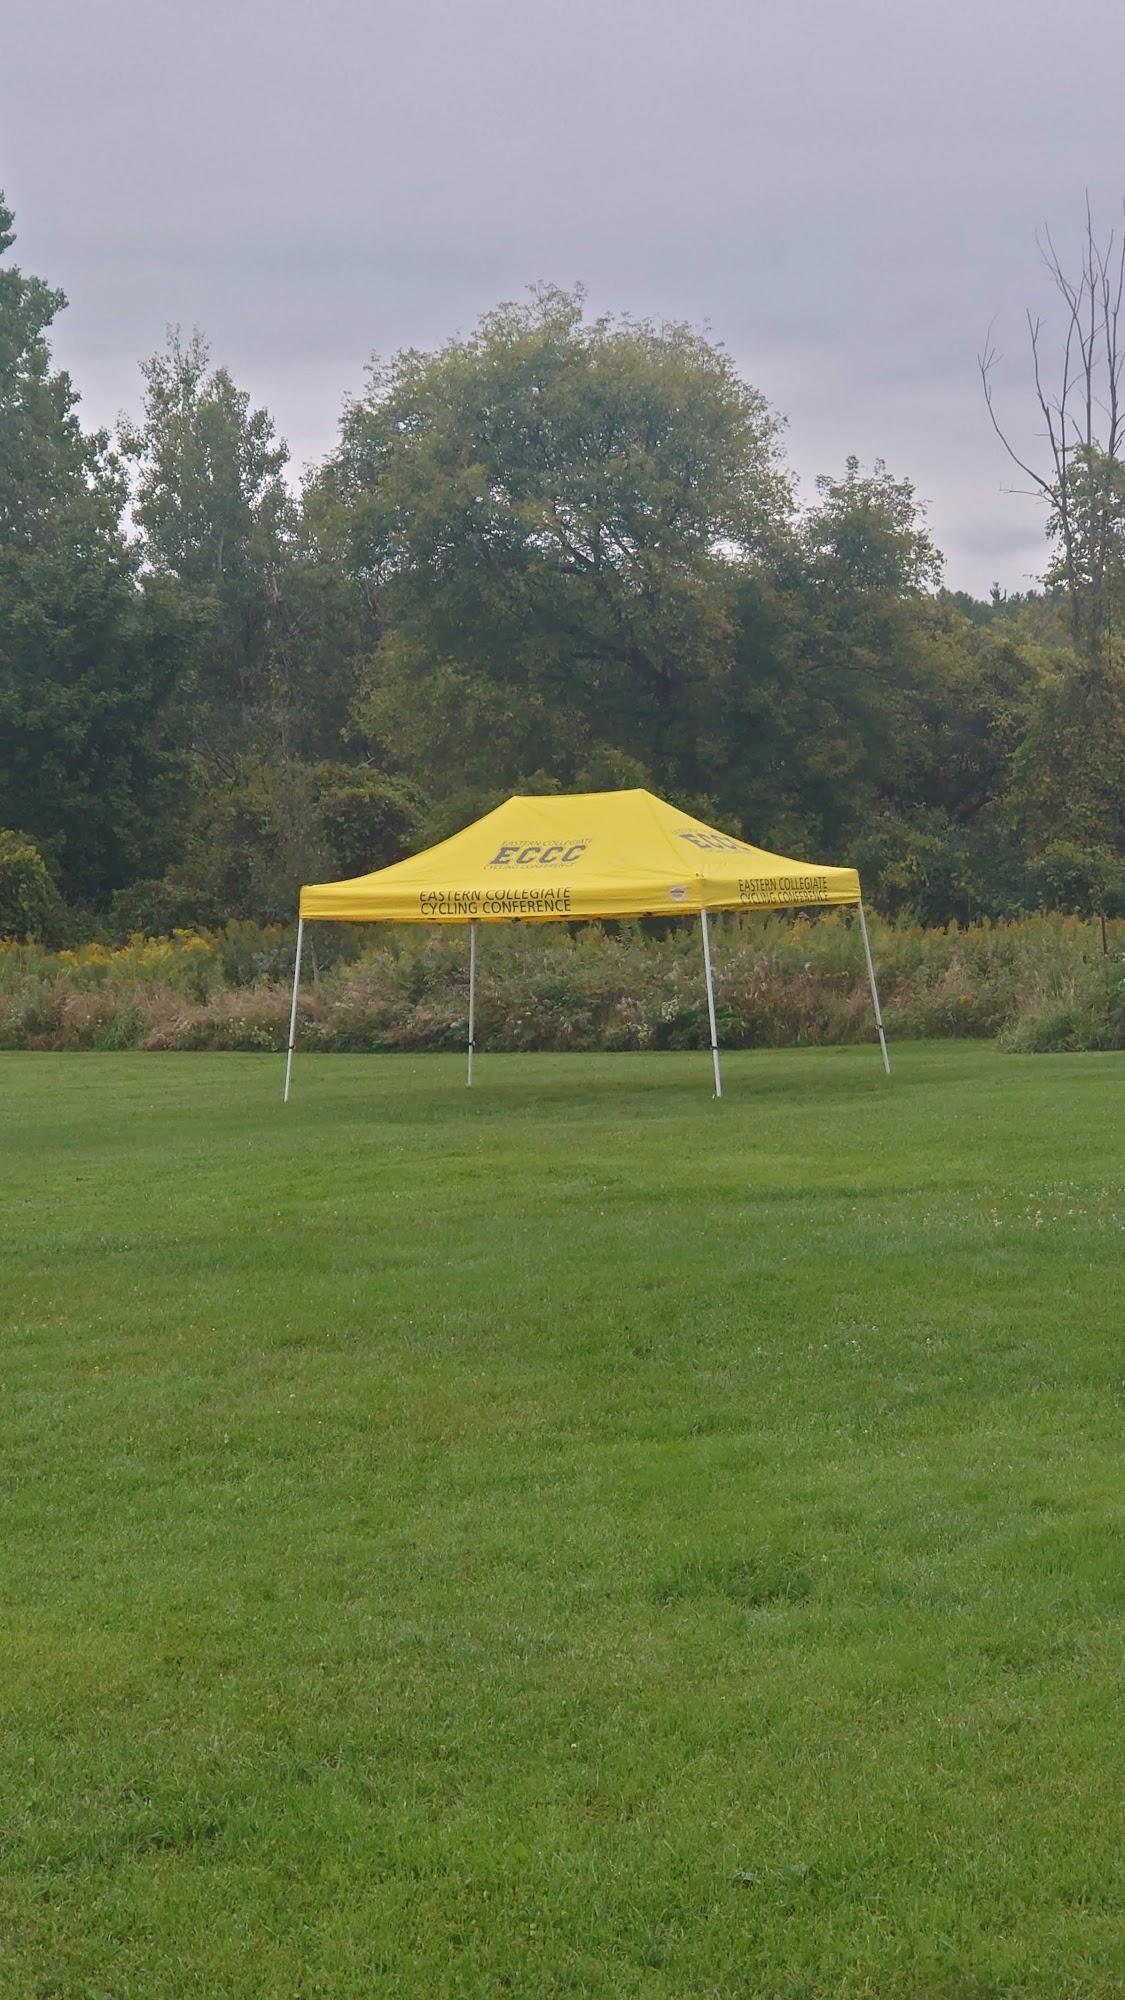
\includegraphics{eccc_tent.jpg}
\caption[The ECCC Tent]{The ECCC Tent\\
          Credit: Flyyn Leonard}
\labfig{eccc_tent}
\end{marginfigure}

If the location of the finish line has not been finalized, pick the location now.
Plan to setup a pop-up tent, table, and chairs at the finish line, unless the officials or timing company are providing their own.

Do a final course inspection:
\begin{itemize}
  \item ensure towing services have removed any cars parked on course
  \item check that navigation signs are in place
  \item check that barriers and signage for locals are in place
  \item look for any course hazards - storm drains, potholes, etc. Cover or mark with spray paint.
  % TODO: document ways to mitigate hazards, reference
\end{itemize}

\index{parking}
Ensure parking is easy to find (put up signs if necessary).
Reserve some parking for event staff.

Mark the finish with a flag, and consider putting down a line - consult with your timing company to ensure your marking does not interfere with the finish line camera.
% TODO: add figure of finish line marking

As staff and volunteers arrive, greet them and fill them in on the essentials, including where restrooms are,
and where registration, the finish line, and staging are going to be.

\index{radios}
If you are using event radios, % TODO: document somewhere, reference
distribute radios early so people already have them before they are needed.
Consider signing out equipment (like radios and safety vests) to reduce the risk of loosing items.

\subsection{Event 1: Criterium}

Most teams will have departed campus sometime Friday afternoon and slept in a hotel or with a local teammate.

About an hour or two before the first race starts,
teams will start parking and making their way to registration.

\subsubsection{Registration}

The majority of riders who come to registration fall into one of the following categories:

\begin{itemize}
  \item Pre-registered riders without a number already,
        who need to check in, turn in any paperwork, and get a number
  \item Riders who have not pre-registered,
        who need to complete waivers and other paperwork,
        pay for their race entry,
        and be assigned a number
  \item Riders who have already been assigned a number,
        but wish to register for additional races
\end{itemize}

% TODO: move the following to a formal registration section, and reference?

However, riders will also use the registration table as their primary location
for any issue, so registration should also be prepared for:

\begin{itemize}
  \item Directing riders to restrooms, staging, feed zones, the finish line, and where results will be posted
  \item Answering questions about which side numbers should be pinned on
  \item Directing any questions about rules to the officials or other staff
  \item Directing riders with minor injuries towards medical, and activating a medical response for any more major incidents that are reported to registration
  \item Directing marshals and other volunteers to the volunteer coordinator, or directly handing out safety vests, flags, and radios
\end{itemize}

\subsubsection{Road Closure}

Typically criterium courses are closed at least 30 minutes before the race starts - this prevents people from parking on course, and provides riders a safe opportunity to pre-ride the course.

\begin{kaobox}[title=Official Pre-Riding and Legal Liabilities]
% TODO: have someone (legal?) review this
\textit{This is not legal advice. Please review laws, insurance documents, USA Cycling regulations, and consult with a lawyer if you have questions.}

If you inform riders that they can pre-ride, either in the permit or verbally, your moral (and potentially legal) responsibilities have started.

Keep safety in mind.

If an injury occurs during an official pre-riding time,
ensure it is fully documented. % TODO: document incident documentation elsewhere, link
\end{kaobox}

\subsubsection{Pre-Riding}
\index{pre-riding}

\subsubsection{Setup}

\begin{enumerate}
  \item Pit
  \item Finish line timing provider
  \item Finish line officials
  \item Lead car/motorcycle (if used)
  \item Medical
\end{enumerate}

\subsubsection{Start Line}

% TODO: mention setting up PA system earlier in document

Roughly 30 minutes % TODO: 30?
before the start of the first race, there should be an announced ``first call to staging''.

\begin{marginfigure}
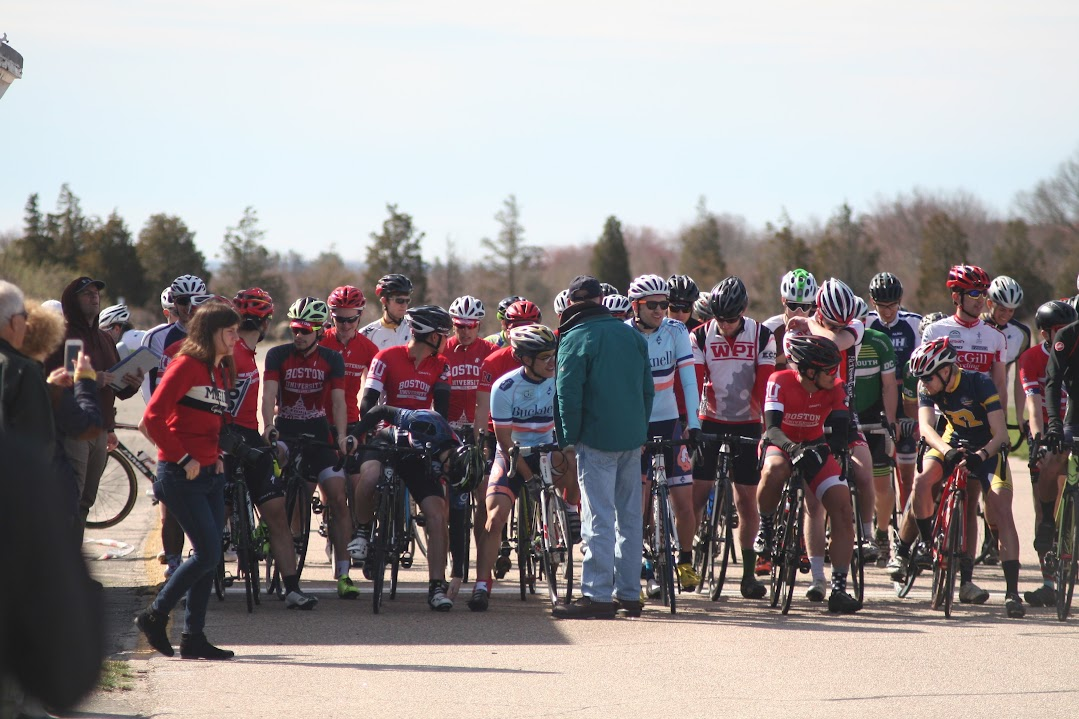
\includegraphics{2017_start_line.jpg}
\caption[Riders lined up at a criterium start line]{
          Riders lined up at the start line for the 2017 Ninigret criterium.\\
          Credit: Flyyn Leonard}
\labfig{criterium_start_line}
\end{marginfigure}

At this point, any lead car or follow official motorcycle should be prepared.
The officials and a race representative should make their way to the staging area/start line.

The chief referee will ensure that they have an official in the pit, and the race organizers should check that marshals are deployed to all corners, course crossings, and any other notable spots.

\subsubsection{Racing}

The whistle blows, and the riders charge off the start line.

% TODO: if start line is a common incident spot, mention

\subsubsection{Beginner's Clinic}

All ECCC criteriums should feature a
beginner's clinic% TODO: document in regulations, link
\sidenote{
Not only do beginners clinics provide the experience we want for new riders,
USA Cycling discounts permitting fees for races that include a beginner's clinic.
}%
.

% TODO: include picture of a clinic

45-60 minutes before the clinic is scheduled to start,
have clinic staff meet and hold a short briefing meeting.
Ensure all clinic staff receive a safety vest.

Inspect the location where the clinic will meet - if one was not picked in advance, quickly find a location at this point.
Ensure the registration table also knows where the clinic will be, as riders frequently ask.

15-30 minutes before the clinic is scheduled to start,
announce the clinic, ensuring to mention where participants should meet.

The clinic should have at least 30-60 minutes of off-course instruction and drills.

Following the drills, the clinic should have a scheduled period when no riders are on course, and the clinic should practice riding around on the course,
and practice cornering on the actual course corners.

This clinic on-course practice time is a good period for the USA Cycling officials and timing company to get a break!

\subsubsection{Beginner Races}

Following the clinic's off-course and on-course sections,
beginner races should be scheduled.

% TODO: include picture of clinic staff

Clinic staff should ride at the back of the beginner race,
providing coaching and support to any riders who need it.

% TODO: Describe the beginner race

\subsubsection{Emergency: Crash}

\subsection{Sunday Morning Setup}

\subsection{Event 2: Time Trial}

\subsection{Event 3: Road Race}

\subsubsection{Marshal Deployment}

\subsubsection{Caravan Preparation}

\subsubsection{Start Line}

\subsubsection{On-Course}

\subsubsection{Emergency: Crash}

\subsubsection{First Rider In}

\subsubsection{Sweep}

\subsection{Course Cleanup}

\section{Post-Event Financial}

\section{Post-Event Paperwork}

\setchapterstyle{kao}
\setchapterpreamble[u]{\margintoc}
\chapter{MTB Race Play-By-Play}
\labch{mtb-play-by-play}

\pagelayout{wide}
\addpart{Regulations}
\pagelayout{margin}

\setchapterpreamble[u]{\margintoc}
\chapter{Race Hosting}
\labch{hosting}

\section{Team-Hosted Events}
\labsec{hosting:team}

There is a long-held expectation in cycling that teams who attend races host events themselves,
contributing to the local racing community.

Teams who successfully organize races:
\begin{enumerate}
  \item provide an opportunity for people to race - if it wasn't for other teams hosting events, you wouldn't get to race yourself
  \item enhance their reputation as a team
  \item have an opportunity to promote their sponsors at the event
  \item have stronger teams by uniting their members in a common project
  \item earn money, via whatever profit is made from the event
\end{enumerate}

Historically, hosting races has been an expectation of collegiate teams as well.

However, recent years have seen a sharp decline in the commitment from teams to run events,
so conferences (including the Eastern Collegiate Cycling Conference) have struggled to run seasons.

For some seasons, the ECCC has started to host their own events, % TODO: hyperlink
and other conferences (such as the SECCC) have had to turn to outside companies to run their seasons, % TODO: hyperlink
increasing costs and sacrificing some of the collegiate atmosphere.

\subsection{Finances and Budget}
\labsubsec{hosting:team:finance}

In a team-hosted race, the organizing collegiate team is responsible for the budget and finances for the race (although the ECCC is here to advise, and has some emergency funds in some circumstances).

The hosting team will be paying for the expenses to run the event:
\begin{itemize}
  \item Venue fees, if applicable
  \item Signage, caution tape, and other course equipment as needed
  \item Permitting fees
  \item Services used at the race, including:
  \begin{itemize}
      \item Officiating
      \item Timing services
      \item Registration services
      \item Medical providers, such as EMTs and bike patrol
      \item Police details
      \item ECCC coordination fees
  \end{itemize}
  \item An ECCC surcharge
\end{itemize}

\subsubsection{ECCC Specific Costs}

There are three areas where money may need to be budgeted as going directly to the ECCC or ECCC staff members.

The exact values that the ECCC charges varies each season - contact your season coordinator and conference director for the current schedule of fees.

\begin{description}
  \item[ECCC Surcharge]
      The ECCC may specify a fixed and/or per-rider expense as an ECCC surcharge, that goes directly to the conference.

      These funds are used to pay for conference equipment that is used at races (including timing equipment, registration equipment, radios, and tents),
      and can also go towards our emergency fund used to prevent schools from loosing too much money hosting races, or to pay for races canceled due to natural disasters or pandemics.
  \item[ECCC Staff Fees]
      The season coordinator, conference director, and associated staff members may charge teams a fee for their work before and during the event.
  \item[ECCC Labor]
      In addition to the work the season coordinator and conference director do to support race organization and oversee the event,
      some events find it most effective to pay ECCC staff members to provide event services in addition to their other duties.

      For example, collegiate mountain weekends typically pay the season coordinator to work as the chief referee in addition to their work running the race day.
\end{description}

\section{Conference-Hosted Events}
\labsec{hosting:conference}

\section{External Races}
\labsec{hosting:external}

\section[Professionally Hosted]{Professionally Hosted Races or Series}
\labsec{hosting:pro}

\setchapterpreamble[u]{\margintoc}
\chapter{Race Formats}
\labch{formats}

In general, the Eastern Collegiate Cycling Conference
runs event disciplines and formats that are specified and defined by USA Cycling.

This section lists several event formats including
common formats seen in the ECCC, however there are additional
formats that could be considered.

\section{Road Events}

Each ECCC road season weekend traditionally runs three events:

\begin{itemize}
  \item A long-format race (see \nrefsubsec{format:rr})
  \item A shorter-format race, such as a criterium (see \refsubsec{format:crit})
  \item A time trial,
      commonly an individual time trial (ITT)
      or a team time trial (TTT),
      but could also be a hill climb (\refsubsec{format:hill_climb})
\end{itemize}

Either the road race or criterium could be replaced by a circuit race (\refsubsec{format:circuit}) if the roads are more suitable for that format.

\subsection{Criterium}
\labsubsec{format:crit}

\subsection{Road Race}
\labsubsec{format:rr}

\subsection{Circuit Race}
\labsubsec{format:circuit}

\subsection{Time Trial}

\subsection{Hill Climb}
\labsubsec{format:hill_climb}

Hill climbs are point-to-point individual time trials that have a significant gain in elevation.

\section{MTB Events}

Each ECCC mountain bike season traditionally contains five events:

\begin{itemize}
  \item Two cross-country races:
  \begin{itemize}
      \item One long distance Cross-Country (XC) race (\refsubsec{format:xc})
      \item One Short-Track Cross-Country (STXC) race (\refsubsec{format:stxc})
  \end{itemize}
  \item A team relay race (\refsubsec{format:relay})
  \item Two gravity races, which can be any of:
  \begin{itemize}
      \item Downhill (DH) (\refsubsec{format:dh})
      \item Dual Slalom (DS) (\refsubsec{format:ds})
      \item Enduro (\refsubsec{format:enduro})
      \item Super Downhill (Super-D) (\refsubsec{format:superd})
  \end{itemize}
\end{itemize}

\subsection{Cross-Country}
\labsubsec{format:xc}

Cross-Country mountain bike races are long-distance races,
timed and run similarly to road races. % TODO: link to road race

\subsection{Short-Track Cross-Country}
\labsubsec{format:stxc}

\begin{marginfigure}
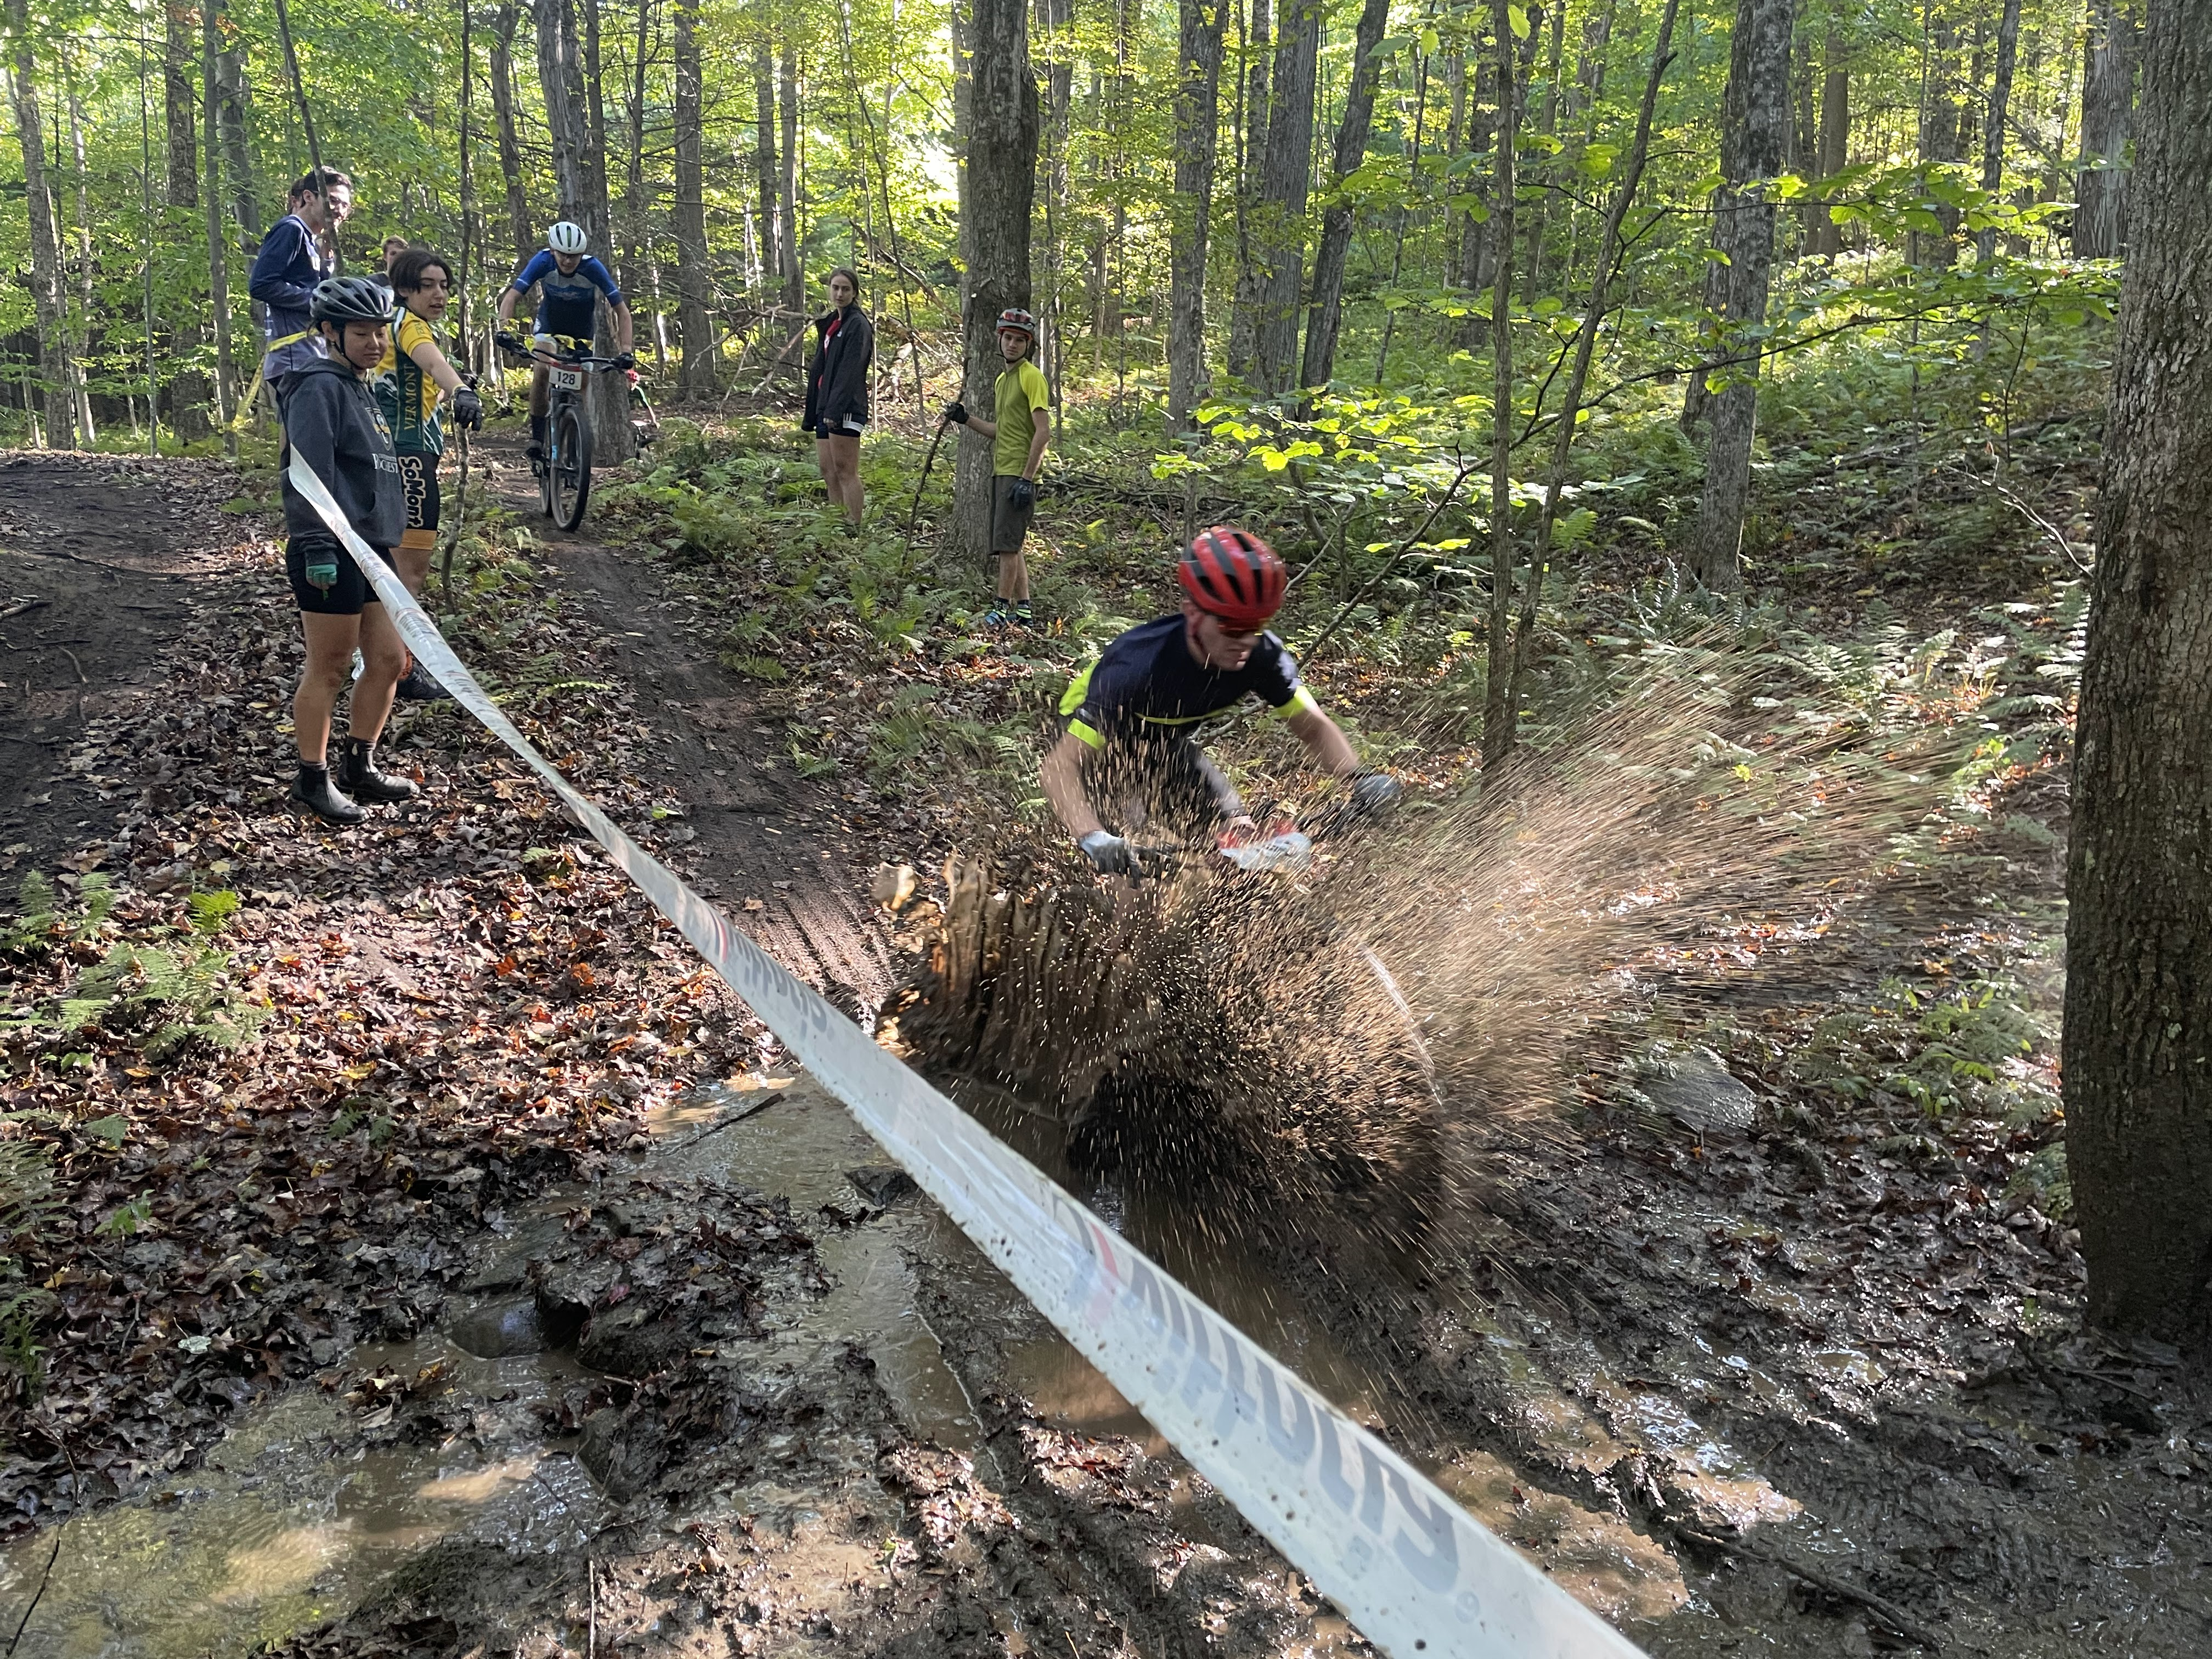
\includegraphics{IMG_9720.jpg}
\caption[A Short-Track Cross-Country Race]{A Short-Track Cross-Country Race.\\
          Credit: Cory Puckett}
\labfig{stxc}
\end{marginfigure}

Short-Track Cross-Country races are the off-road equivalent
to a criterium. % TODO: link to criterium

\subsection{Team Relay}
\labsubsec{format:relay}

Team relay races are team events, typically using the same race course as the Short-Track Cross-Country race, and are often scheduled as following the last STXC field.

\subsection{Dual Slalom}
\labsubsec{format:ds}

Dual Slalom races are short, downhill races that occur on similar, parallel courses.

\subsection{Downhill}
\labsubsec{format:dh}

\subsection{Enduro}
\labsubsec{format:enduro}

\subsection{Super-Downhill}
\labsubsec{format:superd}

\section{Cyclocross Events}

\section{Track Events}

\section{Gravel Events}

\setchapterpreamble[u]{\margintoc}
\chapter{Race Services}
\labch{services}

\section{Medical Services}
\index{EMT}

Every race should have a plan for medical emergencies
which typically includes hiring an EMT % TODO: "EMT" glossary
for event standby services, % TODO: put "event standby services" in glossary and/or markup?
having bike/ski patrol at the event,
or otherwise having someone with medical knowledge on alert.

\begin{kaobox}[title=Local EMT Knowledge]
Flyyn Leonard % TODO: macro for inserting position, e.g. \reftitle{flyyn} => Flyyn Leonard (Conference Director)?
is an EMT
and can help with questions event organizers may have
regarding medical services.
\end{kaobox}

\begin{marginfigure}
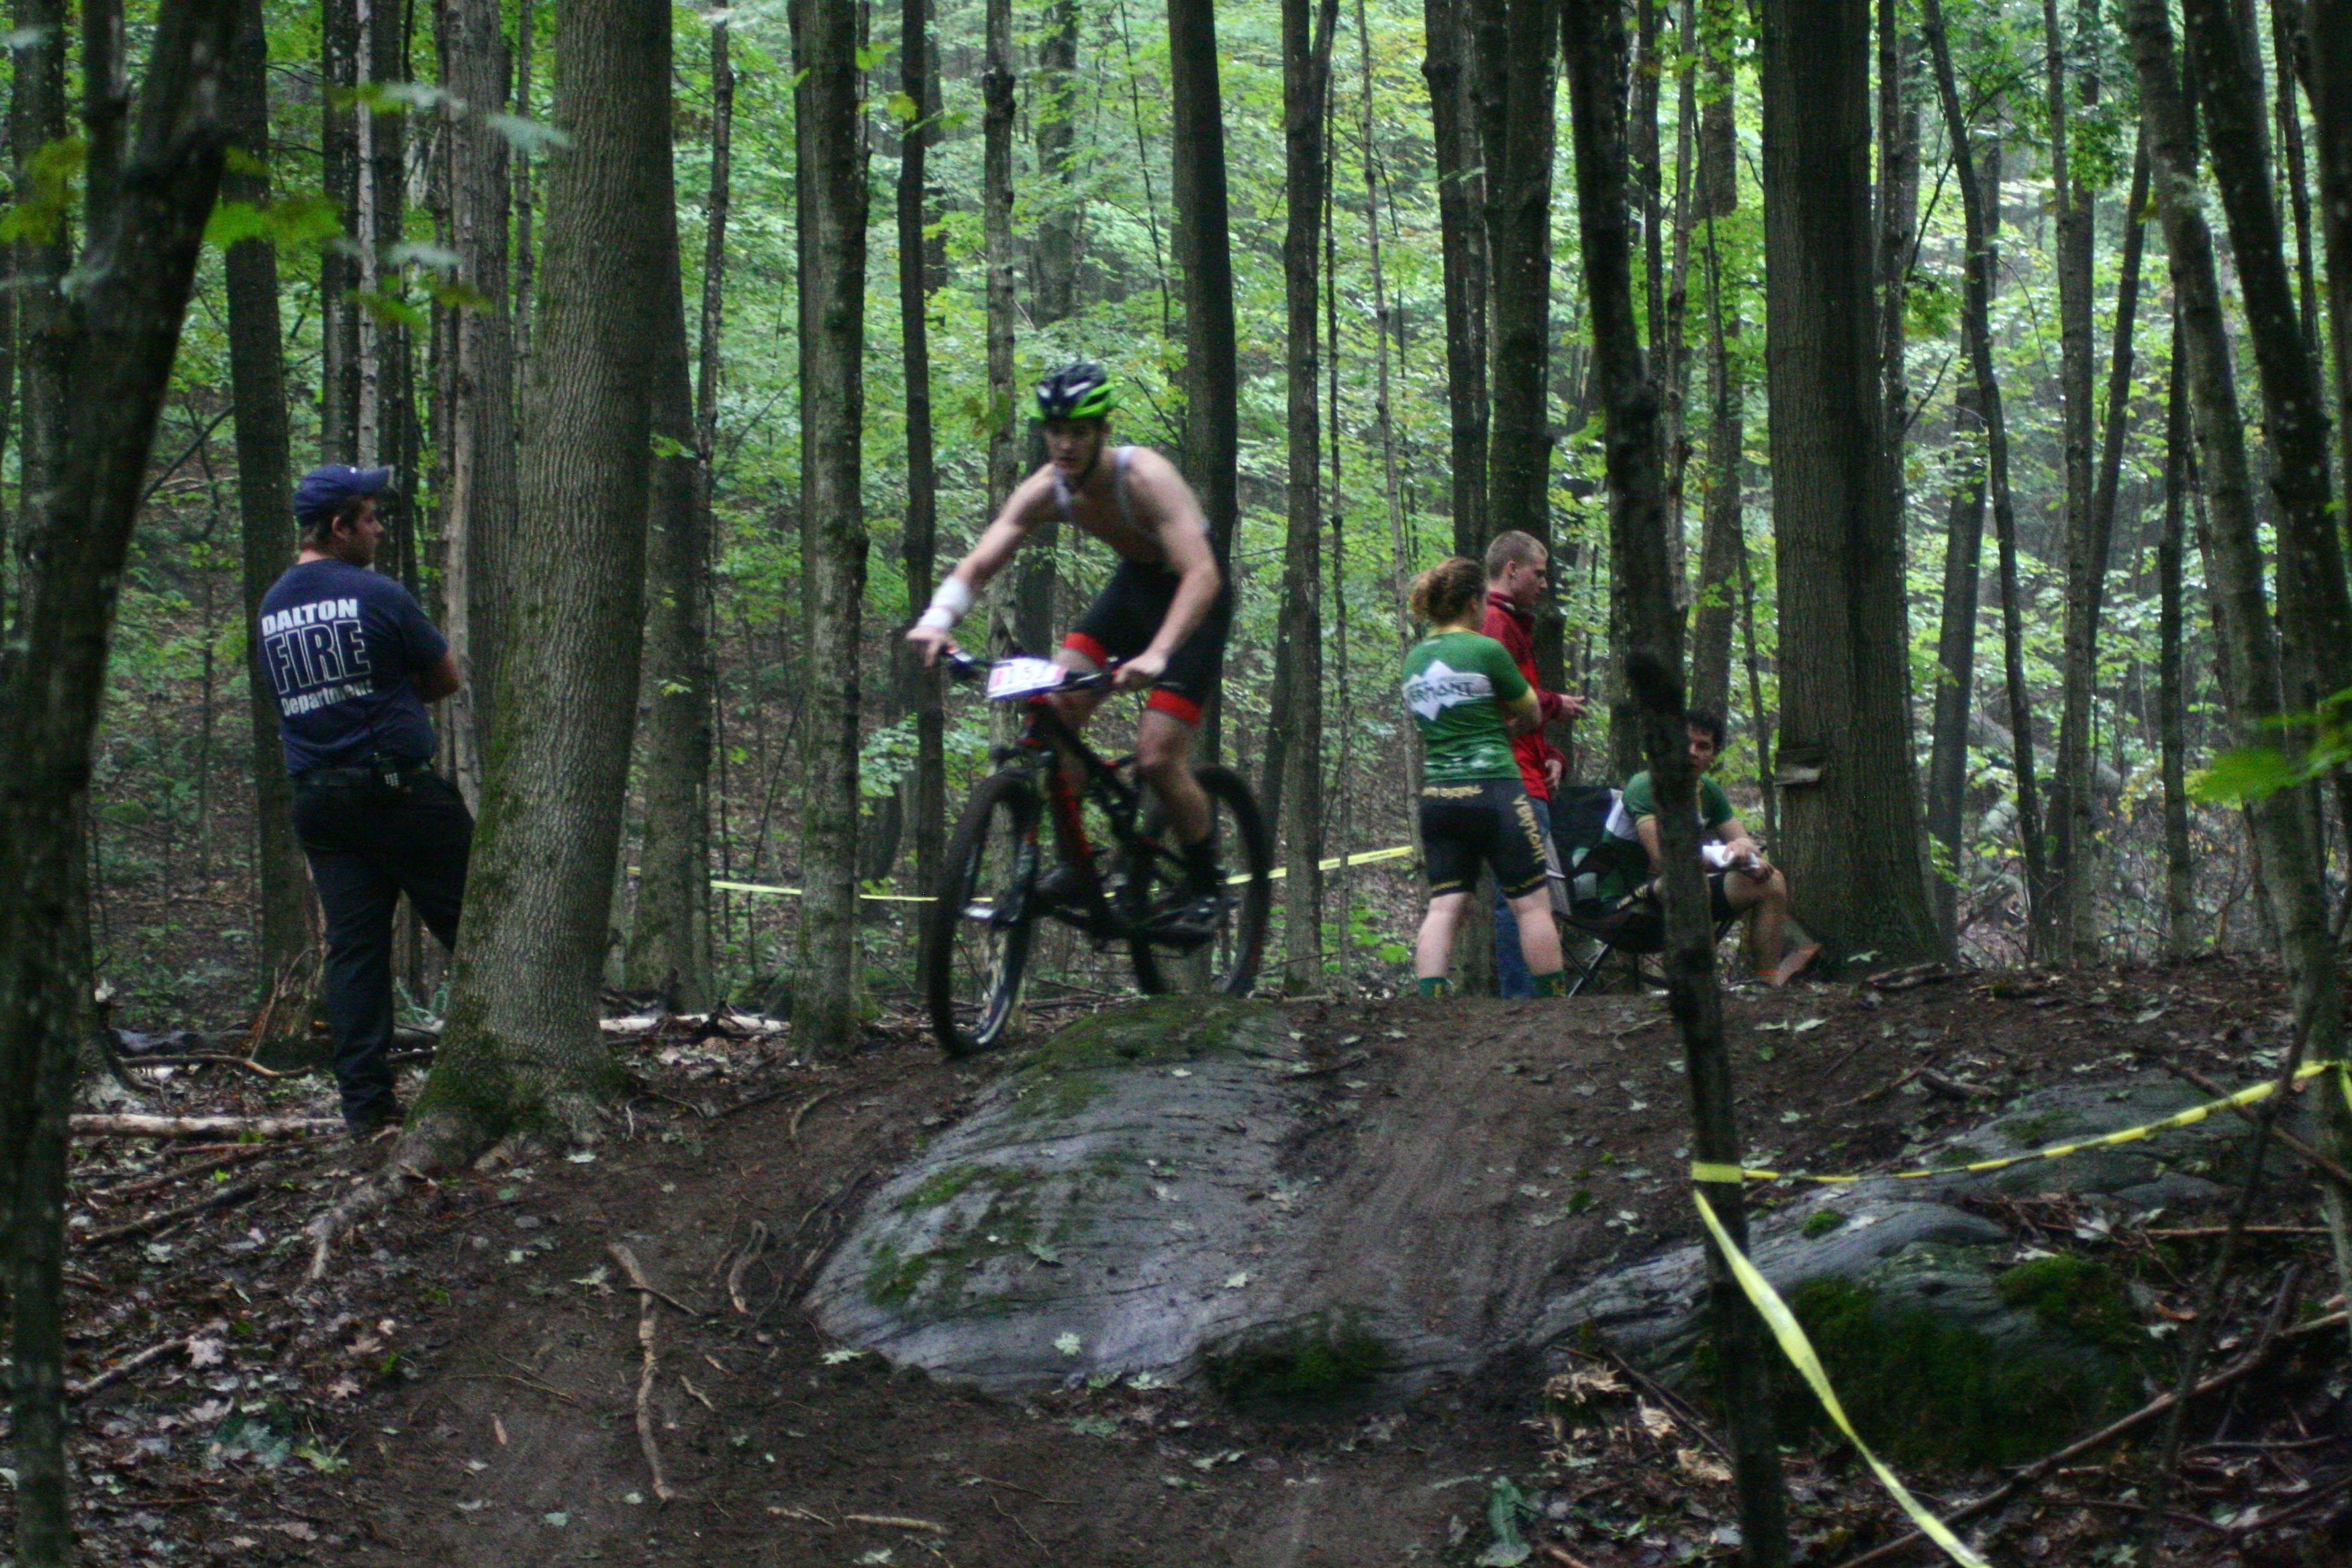
\includegraphics{IMG_5836.jpg}
\caption[Medical Standby]{A member of the Dalton Fire Department on a medical standby detail.\\
          Credit: Flyyn Leonard}
\labfig{standby}
\end{marginfigure}

% \nameref{regulation:medical}

\begin{regulation}[
  ref=medical,
  title=Required Medical Services at ECCC Races,
  draft=true
]
\begin{enumerate}[label=\Alph*.]
  \item
    All ECCC races must make every effort to obtain one or more
    properly licensed, on-duty medical providers (EMT, Advanced EMT, or Paramedic)
    who will be at the race throughout all events.
  \item
    All ECCC races must have at least one person focused on providing first-aid who has some medical or first-aid training.
    This person may be an on-duty member of a bike patrol program, an off-duty EMT, or someone who has completed a Wilderness First Responder course.
\end{enumerate}
\end{regulation}

\subsection{EMS Legal}

\subsection[Contracting]{Contracting EMS Services}

\subsection[EMS Coordination]{Coordination with EMS Providers}

You should request that your medical providers (e.g. EMTs)
arrive at the event before the first race starts -
this ensures the race can start with medical services available,
and gives the promoter time to connect and coordinate with the specific EMT
that covers the event.

You should not expect EMTs to have knowledge of the schedule, event details, or
know anything about bike racing or sports in general.

You should provide EMTs with a schedule of the day and a flyer with basic information
and an event radio (or some other way to communicate with marshals and event staff).
You may also want to provide a quick fact sheet specifically for EMTs - an example is in
\nrefch{med_guide}.

\subsection{Documentation and HIPAA}
\index{HIPAA}

\section{Officiating Services}
\index{officiating}

Officials are essential to an event.
% TODO: description of how

If your event is sanctioned % TODO: glossary
under USA Cycling
you must have a certain number of qualified USA Cycling officials working.

\subsection{Required Officials}

The number of officials varies based on the event and format.

\subsubsection{Mountain Officiating}

\begin{marginfigure}
\includegraphics[angle=270]{PXL_20211003_160518310.jpg}
\caption[MTB STXC Finish Line]{
          A Short-Track Cross Country % TODO: ref
          finish line can be run with a very small crew.\\
          Credit: Katie Aman}
\labfig{standby}
\end{marginfigure}

ECCC MTB races can typically get by with just one chief referee
(traditionally the season coordinator, e.g. Flyyn Leonard)
and a second official or timing assistant,
although additional help is always appreciated.

\begin{kaobox}[title=Note for Team-Hosted MTB Races]
You will need the following officiating resources:

\begin{itemize}
  \item Budget for a USA Cycling Chief Referee (typically Flyyn Leonard)
  \item Budget for a USA Cycling Chief Judge (or otherwise have an experienced official)
  \item Plan to have two volunteers as assistant timers for most events
\end{itemize}
\end{kaobox}

\section{Timing Services}

\section{Registration Services}

\section{Police Services}
\index{police}

\setchapterpreamble[u]{\margintoc}
\chapter{Roles}
\labch{roles}

\pagelayout{wide}
\addpart{Participant Guide}
\pagelayout{margin}

\pagelayout{wide}
\addpart{Team Hosting Guide}
\pagelayout{margin}

\setchapterpreamble[u]{\margintoc}
\chapter{Overview of Team Hosting}
\labch{team_host_overview}

\begin{kaobox}[title=Scope]
This section focuses on
Team-Hosted Events % TODO: properly reference, but name-first style
for road and mountain bike seasons.

Some of the items in the following chapters will only be applicable
for either road or mountain events - for example, ECCC MTB races are typically
officiated by the season coordinator with some assistants, instead of hiring an
entire USA Cycling officiating team.
Sections that are only applicable to certain types of events will be noted as such.

For conference hosted events % TODO: properly reference
please see \nrefch{conference_event:overview},
which focuses on specifically the parts of race organizing
that will be delegated to teams.
\end{kaobox}

\section{Introduction}

Thank you for your interest in hosting a race -
teams hosting races is essential for a healthy cycling community,
especially in collegiate cycling%
\sidenote{This is discussed in detail in \nrefsec{hosting:team}}.

In general, hosting a race is moderately straightforward:
you design a race, fill out paperwork, hire services.
Riders show up, you organize marshals, then registration, officials,
and the timing company run most of the racing.
After that, there's just cleanup and some concluding paperwork.

However, there are a lot of tasks to be done,
and there are a lot of hands needed on the day of the race.

Anyone can host a race - there's no special skills needed,
and our ECCC staff and this document will walk you through every step of the way.

Running a successful race can be rewarding in many ways:
\begin{itemize}
  \item You will be giving back to the cycling community,
        specifically assisting collegiate cycling
  \item Running a race can raise funds for your team
  \item Event organization is a success that you can be proud of (and list on a resume)
\end{itemize}

\section{Steps for Success}

\subsubsection{Divide the load}
Given the number of tasks that must be done, the most successful races often
utilize a large group of people to help spread the work out.

If you are on a large cycling team you may immediately have all the hands you need.
Otherwise if you are on a smaller team, you may want to reach out to teams at other colleges, or even get assistance from local non-collegiate teams.

Consider getting assistance from other sports or outdoor clubs at your school.

\subsubsection{Ask for help}

\subsubsection{Stay ahead of deadlines}

\subsubsection{Confirm everything}

Even members of our ECCC team have made assumptions about
race courses, volunteer commitments, and availability of resources provided by contracted companies.

Even if you've paid to rent a ski mountain for a downhill race,
confirm that they will have members of ski patrol handing medical standby.

\subsubsection{Have contingency plans}

Imagine it is mid-day on Friday, with only a few hours before the first race of the day on Saturday.
The local fire department, who you contracted to provide medical standby services,
calls and informs you that they are unavailable, because they must attend an emergency drill at the local airport.

\section{Responsibilities}

\pagelayout{wide}
\addpart{Assisting with Conference Events}
\pagelayout{margin}

\setchapterpreamble[u]{\margintoc}
\chapter{Overview}
\labch{conference_event:overview}

\pagelayout{wide}
\addpart{The Eastern Collegiate Cycling Conference}
\pagelayout{margin}

\setchapterpreamble[u]{\margintoc}
\chapter{Conference Staff}
\labch{staff}

\appendix

\pagelayout{wide}
\addpart{Appendix}
\pagelayout{margin}

\setchapterpreamble[u]{\margintoc}
\chapter{Event Hosting Document / To-Do List}

\setchapterpreamble[u]{\margintoc}
\chapter{Event Hosting Task Schedule}

\setchapterpreamble[u]{\margintoc}
\chapter{Example Event Budget}

\setchapterpreamble[u]{\margintoc}
\chapter{Road Marshalling Guide}

\setchapterpreamble[u]{\margintoc}
\chapter{Off-Road Marshalling Guide}

\setchapterpreamble[u]{\margintoc}
\chapter{Medical Provider Guide}
\labch{med_guide}

\setchapterpreamble[u]{\margintoc}
\chapter{Police Guide}

\setchapterpreamble[u]{\margintoc}
\chapter{Lead Car Guide}


\setchapterpreamble[u]{\margintoc}
\chapter{USA Cycling Official Handout}

\backmatter
\setchapterstyle{plain}

% TODO: print bibliography
% TODO: print nomenclature
% TODO: print glossary

\printindex

% TODO: print back cover?

\end{document}
